\documentclass[parskip=full]{scrartcl}
\usepackage[top=2.5cm, bottom=2.5cm, left=2.5cm, right=2.5cm]{geometry}
\usepackage[utf8]{inputenc}
\usepackage[T1]{fontenc}
\usepackage[german]{babel}
\usepackage{hyperref}
\usepackage[toc, nonumberlist]{glossaries}
\usepackage{graphicx}
\usepackage{enumitem}
\usepackage{float}
\usepackage{color}

\title{OSIP - Softwaredesign}
\subtitle{OPC UA Simulator for Industrial Plants}
\author{
    M. Armbruster\\
    D. Kahles\\
    H. Lehmann\\
    M. Schwarzmann\\
    N. Wilhelm
}

\begin{document}
\maketitle

\vspace{20px}
\begin{center}
  
\includegraphics[scale=0.4]{../icon.png}
\end{center}
\pagebreak
\tableofcontents
\pagebreak

\section{Einleitung}
OSIP ist in drei große Pakete gegliedert: Simulation, Monitoring und Core.
Simulation realisiert die Fertigungssimulation und Monitoring die Überwachungskonsole.
Core beinhaltet gemeinsame Unterpakete vom Fertigungssimulation und Monitoring sowie Unterpakete zu IO und der Implementierung
von OPC UA.
Das grundlegende Entwurfsmuster Model-View-Controller (MVC) ist bis auf das Model zweifach für die Fertigungssimulation und die Überwachungskonsole verwirklicht, die getrennt von einander existieren.
Das gemeinsame Model befindet sich in Core. Dabei benutzt die Überwachungskonsole nur core.base und core.behavior.
Die Fertigungssimulation benutzt ein erweitertes Model aus den Unterpakteten core.simulation, core.base und core.behavior.
Das Unterpaket core.simulation ist für das Mischen von Farben und die Simulation der Verbindungsrohre zuständig.

\section{Klassenbeschreibungen}
Die Klassenbeschreibungen können im Anhang dieses Dokuments gefunden werden.

\section{Abläufe}
Im Folgenden werden Sequenzdiagramme für typische Aktionen innerhalb von OSIP aufgezeigt und beschrieben.
\subsection{Wrapper für OPC UA}
OSIP verwendet einen Wrapper für Milo, da Milo eine zu komplexe Schnittstelle bereitstellt.
Viele der angebotenen Funktionen (wie beispielsweise mehrere Namespaces) werden von uns nicht benötigt
und werden durch den Wrapper verborgen.


\subsubsection{Server-Wrapper}
\begin{figure}[H]
  \centering
  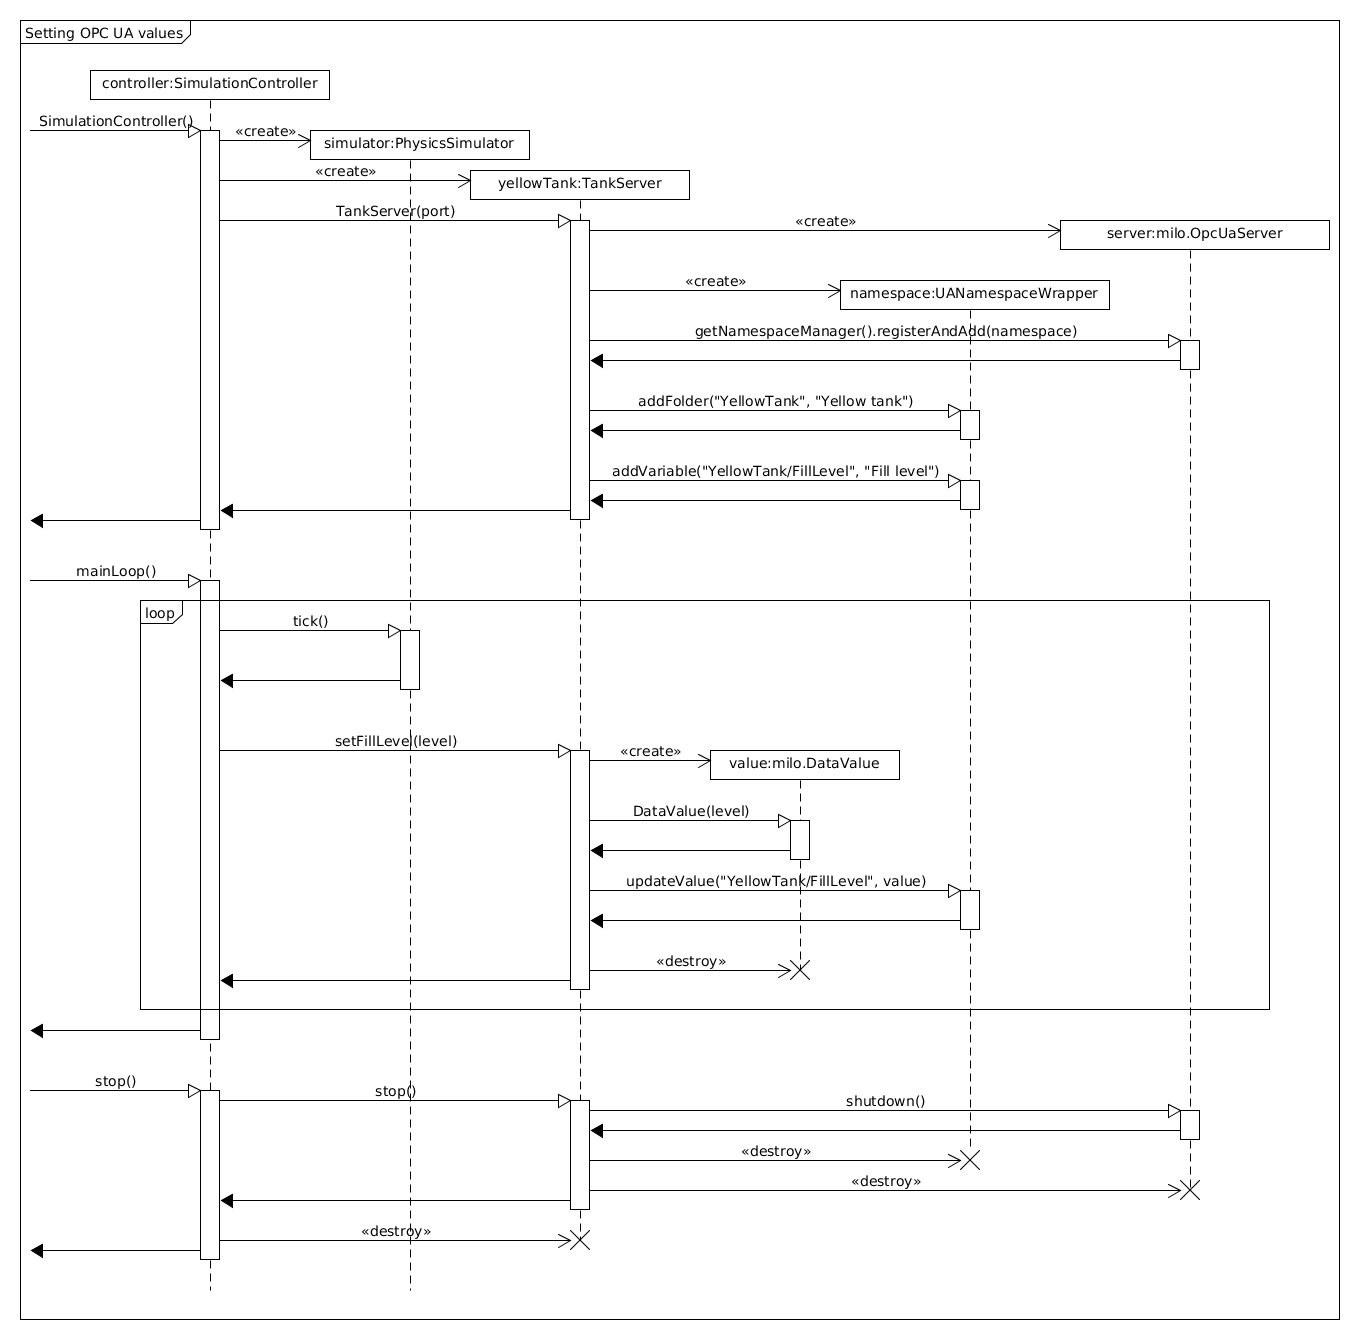
\includegraphics[scale=0.38]{design/sequence-diagrams/sequence-set-server-value.png}
  \caption{Setzen von Werten über den UAServerWrapper}
\end{figure}
Beim Erstellen des Controllers werden auch der Simulator und die Server der Tanks erstellt.
Dieser Server erbt von \emph{UAServerWrapper}, welcher eine Abstraktion von Milo vornimmt. Wie im Diagramm zu sehen,
werden vom Wrapper Server und Namespace erstellt. Der Namespace wird beim Server registriert und
im Namespace werden die Ordner und Variablen erstellt (hier exemplarisch der Füllstand).

Beim Setzen des Füllstandes wird nur \emph{setFillLevel()} aufgerufen. Der \emph{UAServerWrapper} erstellt daraufhin
ein entsprechendes \emph{DataValue}, das von Milo gebraucht wird, und übergibt es an den Standard-Namespace.
Durch einen Aufruf von \emph{stop()} fährt der \emph{UAServerWrapper} den Server herunter und dereferenziert
Server und Namspace.

\subsubsection{Client-Wrapper}
\begin{figure}[H]
  \centering
  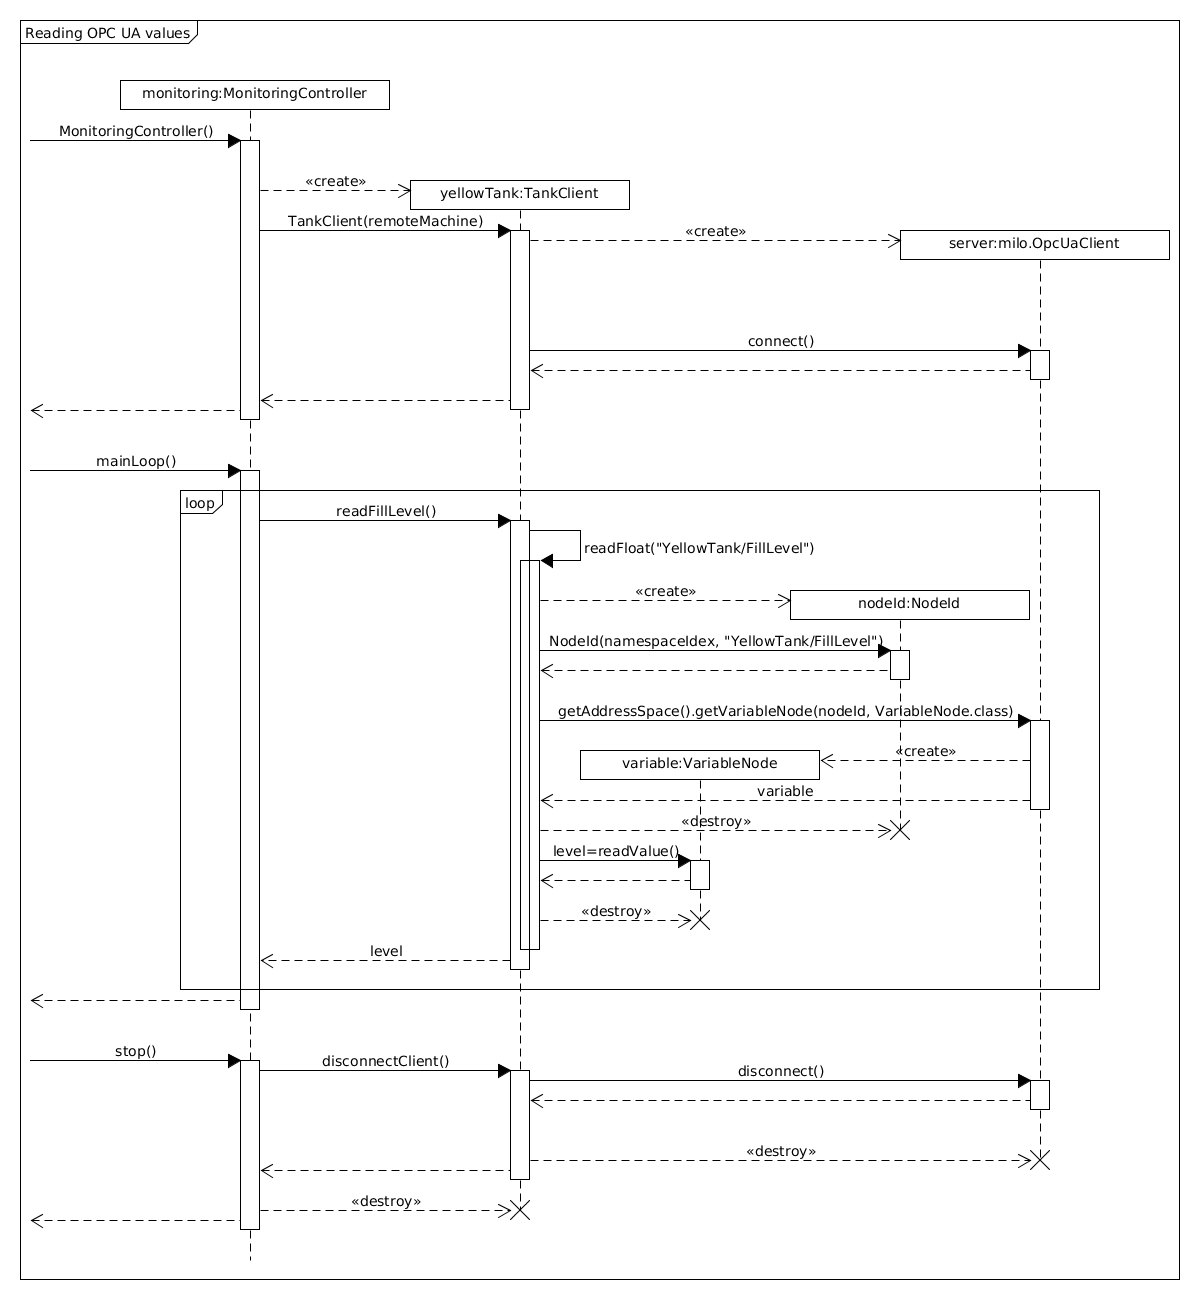
\includegraphics[scale=0.4]{design/sequence-diagrams/sequence-read-client-value.png}
  \caption{Lesen von Werten über den UAClientWrapper}
\end{figure}
Der Controller ruft beim \emph{TankServer}, welcher von \emph{UAClientWrapper} erbt, die read-Methode für den entsprechenden Parameter auf
(hier exemplarisch \emph{readFillLevel()}). Der \emph{UAClientWrapper} erstellt ein \emph{NodeId}-Objekt und ruft damit
vom Client die entsprechende \emph{VariableNode} ab. Von dieser \emph{VariableNode} wird nun schlussendlich der Wert abgerufen.
Dieser Wert wird zurück an den Controller gegeben. Der \emph{UAClientWrapper} übernimmt somit die
komplette Interaktion mit Milo.

\subsection{Neuzeichnen der GUI der Simulation}
\begin{figure}[H]
  \centering
  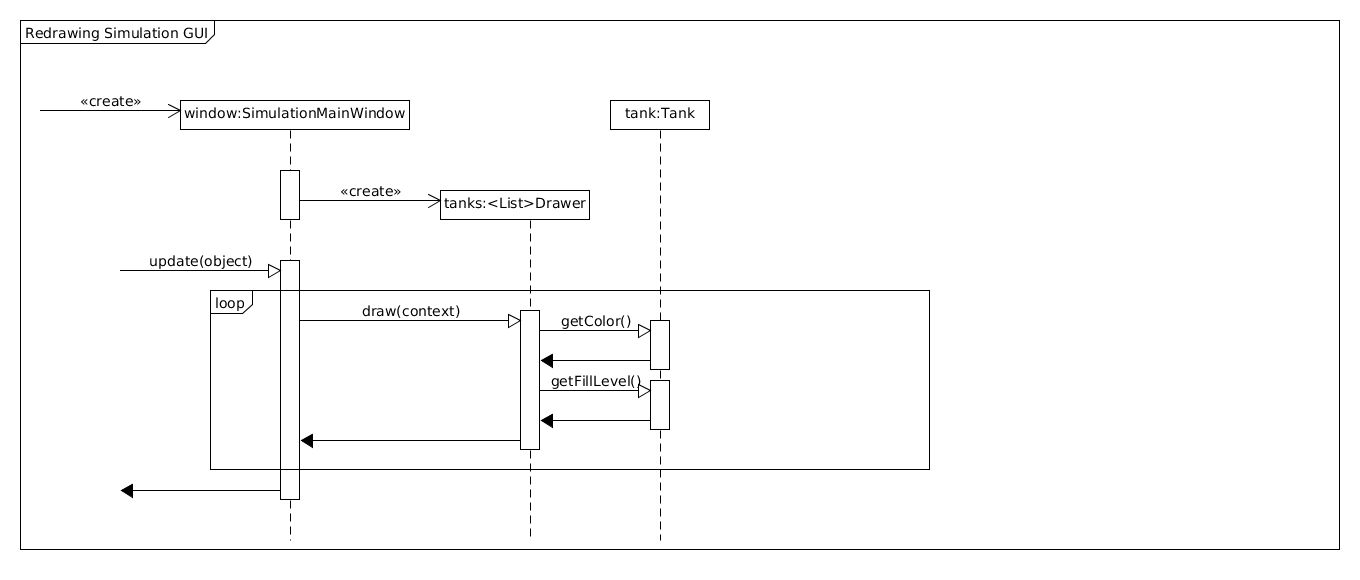
\includegraphics[scale=0.35]{design/sequence-diagrams/simulation-redraw.png}
  \caption{Neuzeichnen der GUI der Simulation}
\end{figure}

\subsection{Berechnen der Tank-Simulation}
\begin{figure}[H]
  \centering
  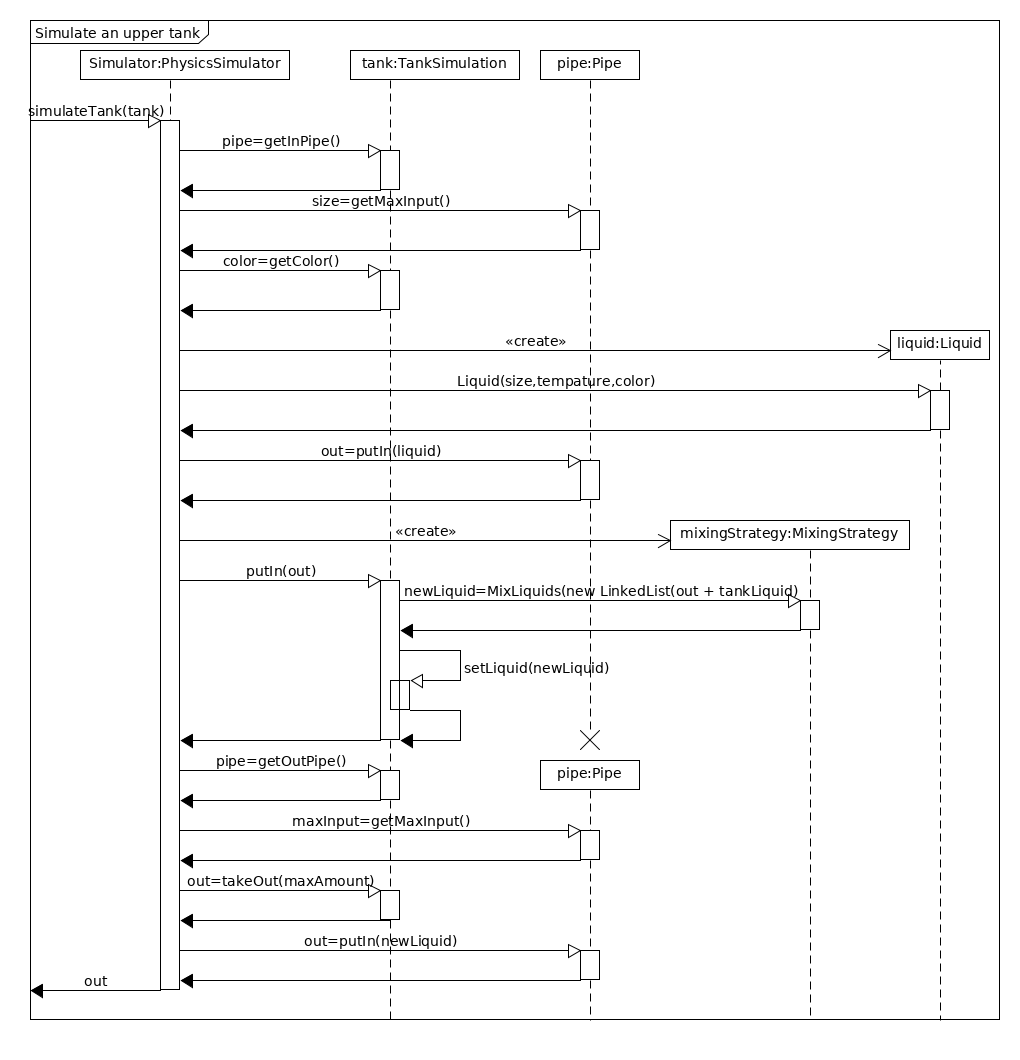
\includegraphics[scale=0.45]{design/sequence-diagrams/tank-simulation.png}
  \caption{Berechnen der Tank-Simulation}
\end{figure}
Dies ist die Simulaiton eines der oberen Tanks. Für die vollständige Simulation, muss \emph{simulateTank()} für jeden Tank aufgerufen werden,
und die Rückgabewerte zum Mixtank hinzugefügt werden. Zuerst erfrägt die Simulation beim Tank die Leitung, die zum Tank hinführt, und ermittelt
mit \emph{getMaxInput()} die maximale Durchflussmenge. Anschließend wird die noch im Tank enthaltene Flüssigkeit geholt, um dessen Farbe zu bestimmen.
Dann kann ein neues \emph{Liquid} Objekt erstellt werden, das so groß ist, das es gerade noch in die Leitung passt. Mittels \emph{putIn} wird es
in die Leitung gesteckt. Der Rückgabewert von \emph{putIn} ist die Flüssigkeit, die am anderen Ende der Leitung herauskommt. Diese wird dann in den
Tank eingefügt. Dazu verwendet der Tank eine \emph{SubtractiveMixingStrategy} um die Farben und Temperaturen zu mischen. Nachdem die Flüssigkeiten
gemischt sind, wird die Leitung vom oberen Tank zum Mixtank geholt, und ermittelt, wie viel Flüssigkeit dort hineinpasst. Diese Menge wird dann aus dem
Tank herausgenommen, und in diese Leitung hineingesteckt. Der Rückgabewert von \emph{simulateTank()} ist dann die Flüssigkeit, die am Ende der Leitung
(also beim Mixtank) herauskam. Diese Flüssigkeit kann die Simulation dann in den Mixtank einfügen (nicht mehr in diesem Diagramm dargestellt).

\subsection{Einstellungen aus der Datei erhalten und verwenden}
\begin{figure}[H]
  \centering
  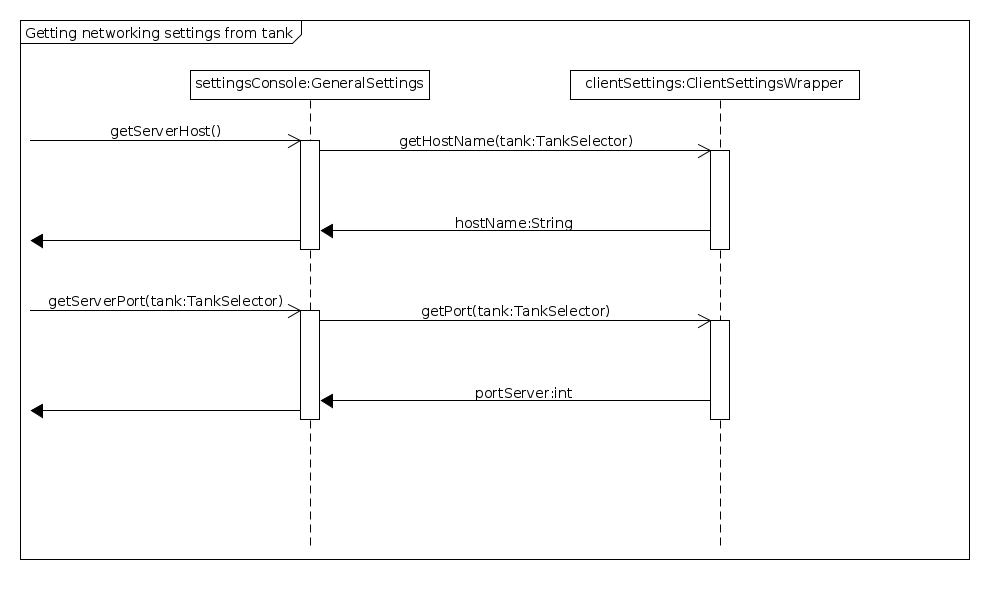
\includegraphics[scale=0.4]{design/sequence-diagrams/getting-networking-settings.png}
  \caption{Einstellungen aus der Datei erhalten und verwenden}
\end{figure}
Bei der Erstellung eines \emph{TankClient} werden Hostname und Port des zugehörigen Servers vom mit \emph{getHostName(tank:TankSelector)}
und \emph{getPort(tank:TankSelector)} vom \emph{ClientSettingsWrapper} abgerufen. Eine Instanz des \emph{ClientSettingsWrapper}s
ist im \emph{MonitoringController} zu finden. Es wird eine \emph{RemoteMachine} erstellt und mit Hostname und Port konfiguriert.
Danach erstellt man einen \emph{TankClient}, der die \emph{RemoteMachine} übergeben bekommt und sich mit dem Server verbinden kann.

\pagebreak
\section{Änderungen zum Pflichtenheft}

\subsection{\"Ubernommene Kann-Kriterien}
Im folgenden werden die Kann-Kriterien aus dem Pflichtenheft noch einmal alle aufgelistet. Zu jedem der Kriterien wird
kurz zusammengefasst, was genau es bedeutet. Es werden erst die implementierten und anschlie{\ss}end die nicht implementierten
Kriterien gelistet.

\subsubsection{Implementierte Kann-Kriterien}
Die implementierten Kann-Kriterien sind wie folgt:

\begin{itemize}
    \item Sowohl in der \"Uberwachungskonsole als auch in der Fertigungssimulation werden Fehler bei der Programmausf\"uhrung
    nach stdout geloggt. Die Logs werden nicht persistiert.
    \item In der Fertigungssimulation k\"onnen vorgefertigte Simulationsszenarien geladen werden. Diese sind in eigenen Dateien definiert.
    Die Ausführung der Simulationsszenarien f\"uhrt dazu, dass die Steuervariablen sich nach Vorgaben des Szenarios ohne
    weitere Aktion des Benutzers \"andern.
    \item In den Zuflusswerten der Fertigungssimulation ist ein Jitter eingebaut. Dieser sorgt f\"ur leichte Variationen in den
    Zuflussmengen und der Temperatur der Zufl\"usse. Das Ausma{\ss} des Jitters ist nicht einstellbar.
    \item Innerhalb der \"Uberwachungskonsole kann der Benutzer selbst einstellen, in welchem Zeitintervall die Werte der
    Fertigungssimulation abgefragt werden. Alle Werte werden im jeweils gleichen Intervall abgefragt.
    \item Die Alarme in der \"Uberwachungskonsole k\"onnen vom Benutzer jeweils einzeln zu- und abgeschaltet werden. Die Menge der
    aktivierten Alarme wird bei Beenden der \"Uberwachungskonsole persistiert. Beim n\"achsten Start der \"Uberwachungskonsole
    werden die gleichen Alarme automatisch wieder aktiviert.
    \item Die Alarme, die von der \"Uberwachungskonsole empfangen werden, werden in einer Textausgabe innerhalb der
    \"Uberwachungskonsole geloggt.
\end{itemize}

\subsubsection{Nicht implementierte Kann-Kriterien}
Die nicht implementierten Kann-Kriterien sind wie folgt:

\begin{itemize}
    \item Es stehen keine verschiedenen Sprachoptionen f\"ur \"Uberwachungskonsole und Fertigungssimulation zur Verf\"ugung.
    Die einzige vorhandene Sprache ist Englisch. Durch die Verwendung von \emph{java.util.ResourceBundle} ist die Anwendung allerdings leicht übersetzbar.
    \item Die vorgegebenen Alarme k\"onnen nicht ver\"andert werden. Insbesondere ist es nicht m\"oglich, eigene Alarme hinzuzuf\"ugen
    oder die Schwellenwerte der vorgegebenen Alarme zu modifizieren.
    \item Der Jitter in den Simulationswerten ist fest vorgegeben und kann in seiner Intensit\"at nicht ver\"andert werden.
    \item Fehler bei der Programmausf\"uhrung werden nicht in eine Datei geschrieben.
\end{itemize}

\section{Klassendiagramme}
Die Klassendiagramme können im Anhang dieses Dokuments gefunden werden.

\pagebreak
\section{Verwendete Entwurfsmuster}
\subsection{Fassaden-Muster: UAServerWrapper, UAClientWrapper}
Milo besitzt eine sehr komplexe Schnittstelle, zu deren Benutzung man sich ausgiebig mit dem oft schlecht dokumentierten Code
der Library beschäftigen muss (Zertifikate manuell deaktivieren etc.). Des Weiteren unterstützt Milo mehr Funktionalität,
als sie in unserem Kontext gebraucht wird (mehrere Namespaces etc.).

Das Fassaden-Muster ist dazu da, um Schnittstellen zu vereinfachen und vereinheitlichen.
Der \emph{UAServerWrapper} erstellt automatisch einen standard namespace und leitet Anfragen an
diesen weiter. Zusätzlich wird das Starten des Servers durch Verstecken von Initialisierungen vereinfacht. Der \emph{UAClientWrapper}
bietet Methoden, um Werte bestimmter Typen direkt und synchron vom Server abzurufen. Die Werte können hierbei direkt über ihren
Namen angesprochen werden - die Umsetzung in \emph{NodeId}s entfällt über die Fassade.

Wir haben das Muster gewählt, um allen
Beteiligten die Handhabung von Milo zu erleichtern. Durch die Fassade muss sich nur noch eine Person damit beschäftigen, wie
Milo intern zu benutzen ist - nicht mehr jeder, der Werte über OPC UA austauschen möchte.

\pagebreak
\phantomsection
\addcontentsline{toc}{section}{\listfigurename}
\listoffigures

\end{document}
